\documentclass[12pt, a4paper]{article}

\usepackage[margin=1.0in]{geometry}

\usepackage{lipsum}% Just for this example
\usepackage{url}
\usepackage{amsmath}
\usepackage{adjustbox}
\usepackage{graphicx}
\usepackage{footnote}
\usepackage{color}
\usepackage{subcaption}
\setlength{\parindent}{0pt}% No paragraph indent
\pagestyle{empty}% No page headers/footers

\renewcommand{\baselinestretch}{1.3}
\setlength{\parskip}{1em}

\author{
	Claudio Bruderer\\
	\texttt{cbruderer@phys.ethz.ch}
	\and
	Andrina Nicola\\
	\texttt{nicolaa@phys.ethz.ch}
	\and
	Anna Weigel\\
	\texttt{anweigel@phys.ethz.ch}
}
\title{Spurious relationships in Twitter data\\
	 	 \large Data Science in Techno-Socio-Economic Systems\\
	 	 \large Spring Semester 2016}

\begin{document}
\date{}
\maketitle

\begin{abstract}

One of the main goals in data analysis of any sort, is detecting and quantifying relations between quantities. With the increasing amount of data available to us, this task becomes more challenging, since large datasets are prone to spurious correlations. It is therefore important to identify these spurious correlations in order to be able to distinguish them from causal relationships. In this project we search for spurious correlations by querying twitter data for a list of pre-defined keywords and computing the correlation between keyword pairs from the time series of the keyword occurrence frequencies. We compute correlations using two separate methods and find that both methods detect expected as well as spurious correlations. These results show that for large datasets, we are easily inclined to over-interpret the results and that conventional correlation measures need to be well understood and carefully applied. 

\noindent Our results are also available online: http://spuriousrelationships.eu.pn/

\noindent All scripts (including \LaTeX$ $ files) used in this analysis are public and can be found here: https://github.com/cbruderer/spuriousrelations/

\end{abstract}


\vspace{0.2in}

\section{Introduction}
We have entered the era of Big Data and the wealth of information available to us entails its own new challenges. Relationships between quantities, whether real or without any obvious causal link, will naturally arise if the data sets are large enough (for examples see \cite{tyler_vigen}). Even though we might be inclined to interpret apparent links between measurements, a correlation does not imply causation. One needs to find a way to distinguish spurious relationships between measurements from those with a causal link, and quantify the frequency of chance correlations occurring.

Based on a list of pre-defined keywords and Twitter data, we aim to show that relationships between quantities without any obvious causal link can be identified in large data sets. 
We use a Twitter dataset which contains unfiltered tweets between May 2014 - July 2014 and September 2014 - December 2014. For each day, we determine the number of tweets containing one of our pre-defined keywords. We then measure and quantify the time-correlation functions between the popularity of various keywords. To test our method we recover and quantify expected correlations between synonyms or related keywords. We  additionally investigate and discuss the performance of different correlation measures.

\section{Data}
\subsection{Data set}\label{sec:data}
In order to identify relationships between words, we need a suitable data set containing a large amount of text data and covering an extended period of time. Data from all major social media platforms primarily using text as a medium (e.g. Twitter \cite{twitter}, Facebook \cite{facebook}, and Reddit \cite{reddit}) satisfy these conditions.

We decided to apply our analysis on Twitter data, which has been previously gathered by an ETH research group. This data set was created via the public Twitter stream \cite{twitterstream}, which downloads 1\% of the tweets posted at that moment without applying any further filtering, and covers the years 2012-2014. We analyse a subset of the whole data set, which contains data of the months May, 2014 - July, 2014 and September, 2014 - December, 2014. These data have been converted to Parquet files, thus simplyfying reading in the data.

\subsection{Keyword selection}

\begin{minipage}{\linewidth}
  \centering
  \captionof{table}{Selected keywords}\label{tab:keywords} 
  \begin{tabular}{ | l | l | l | l | l | }
    \hline
    Terrorism / Religion & Refugees & Ebola & Influenza & Science \\ \hline
    isis & syria & ebola & influenza & bitcoin \\
    terrorism & refugees & guinea & flu & rosetta \\
    arab & migrants & sierra & birds & comet \\
    spring & africa & leone & swine & higgs \\
    attack & italy & liberia & pig & climate \\
    god & ethiopia & virus &  & doomsday \\
    christian & asylum & epidemic &  & maya \\
    allah & unhcr & vaccine &  & curiosity \\
    islam & immigration & who &  & sandy \\
     & foreigners &  &  & hurricane \\ \hline \hline
     
    Discrimination & Countries / Cities & Technology & Everyday life & Food / Trends \\ \hline
    
    black & europe & apple & homework & vegan \\
    white & usa & linux & television & gluten \\
    croweded & philippines & pc & coffee & vegetarian \\
    left & sochi & google & tea & meat \\
    right & olympics & iphone & school & pasta \\
     & geneva & galaxy & work & banana \\
     & boston & watch & teacher & \\
     & london & facebook & sports & \\
     &  & twitter & jogging & \\
     &  & whatsapp &  marathon & \\ \hline \hline
     
    Malaysian Airlines & Ukraine / Crimea & Politics & Family & \\ \hline
    mh17 & ukraine & snowden & family & \\
    mh370 & crimea & nsa & divorce & \\
     & russia & obama & marriage & \\
     &  & putin & wedding & \\
     &  & mandela & holidays & \\
     &  & nelson &  & \\
     &  & pope &  & \\
     &  & unemployment &  & \\
    \hline
  \end{tabular}
  % \par
\end{minipage}

In our analysis we select one hundred keywords. All these keywords are listed in Table~\ref{tab:keywords}. To choose these keywords, we apply different criteria. First, we identify major events that happened during the period for which we have access to twitter data (May 2014 - July 2014 and September 2014 - December 2014). For these topics, we then select related words, and deliberately including synonyms as well. Besides these `major events categories` we also choose words related to long-term trends we {\it a priori} expect to find in the data (e.g. `Food / Trends`, `Refugees`, `Politics`). Furthermore, we include a group of keywords on `Everyday life` for which we {\it a priori} do not expect to see strong trends.

These selection criteria are chosen to address various problems. First, by picking words related to major events localized in time (e.g. Rosetta satellite \cite{rosetta} dispatching Philae lander), we are able to test our pipeline and assert that this {\it a priori} expected quick rise in mentions on social media platforms is identified in our data as well. Second, by including several synonyms, it is reasonable to expect certain correlations between the keywords, hence allowing us to validate our analysis in a second, independent way. Third, the keywords for which we do not {\it a priori} expect the number of mentions to display a significant structure over time (e.g. `Everyday life`), should only weakly correlate with other keywords displaying more structure.

We note however that there are caveats in this type of analysis. Many words have different meanings and could thus potentially correlate or not correlate with other words depending on which meaning is more common. As an example, we include `who` in our analysis. While it is primarily used as a pronoun, it is also the abbreviation of the World Health Organization \cite{who}. Due to the Ebola outbreak in Western Africa in 2014, we expect this secondary meaning to modulate the number of mentions over time, and potentially display correlations with related words (e.g. `ebola`). Other examples of words with multiple meanings include `right` (opposite of wrong; political perspective; direction) and `left` (past participle of leave; political perspective; direction).

\subsection{Data analysis}
We use the \textsc{Python} front end of Apache \textsc{Spark}\cite{pyspark} called \textsc{pyspark} to analyse the twitter data. The data set is read in and then filtered to contain only non-empty tweets. As a next step, the timestamp is adjusted to be in a more accessible format, which encodes only the day of the year and the year, and the tweets are split up into individual words and converted to be only lowercase. For all words we compute jointly the number of mentions per day. As a last step, we filter to only recover the statistics for our keywords, where we also take the keywords into account if they are used as a hashtags, and save the results.

\subsection{Data completeness}
\begin{figure}
\centering
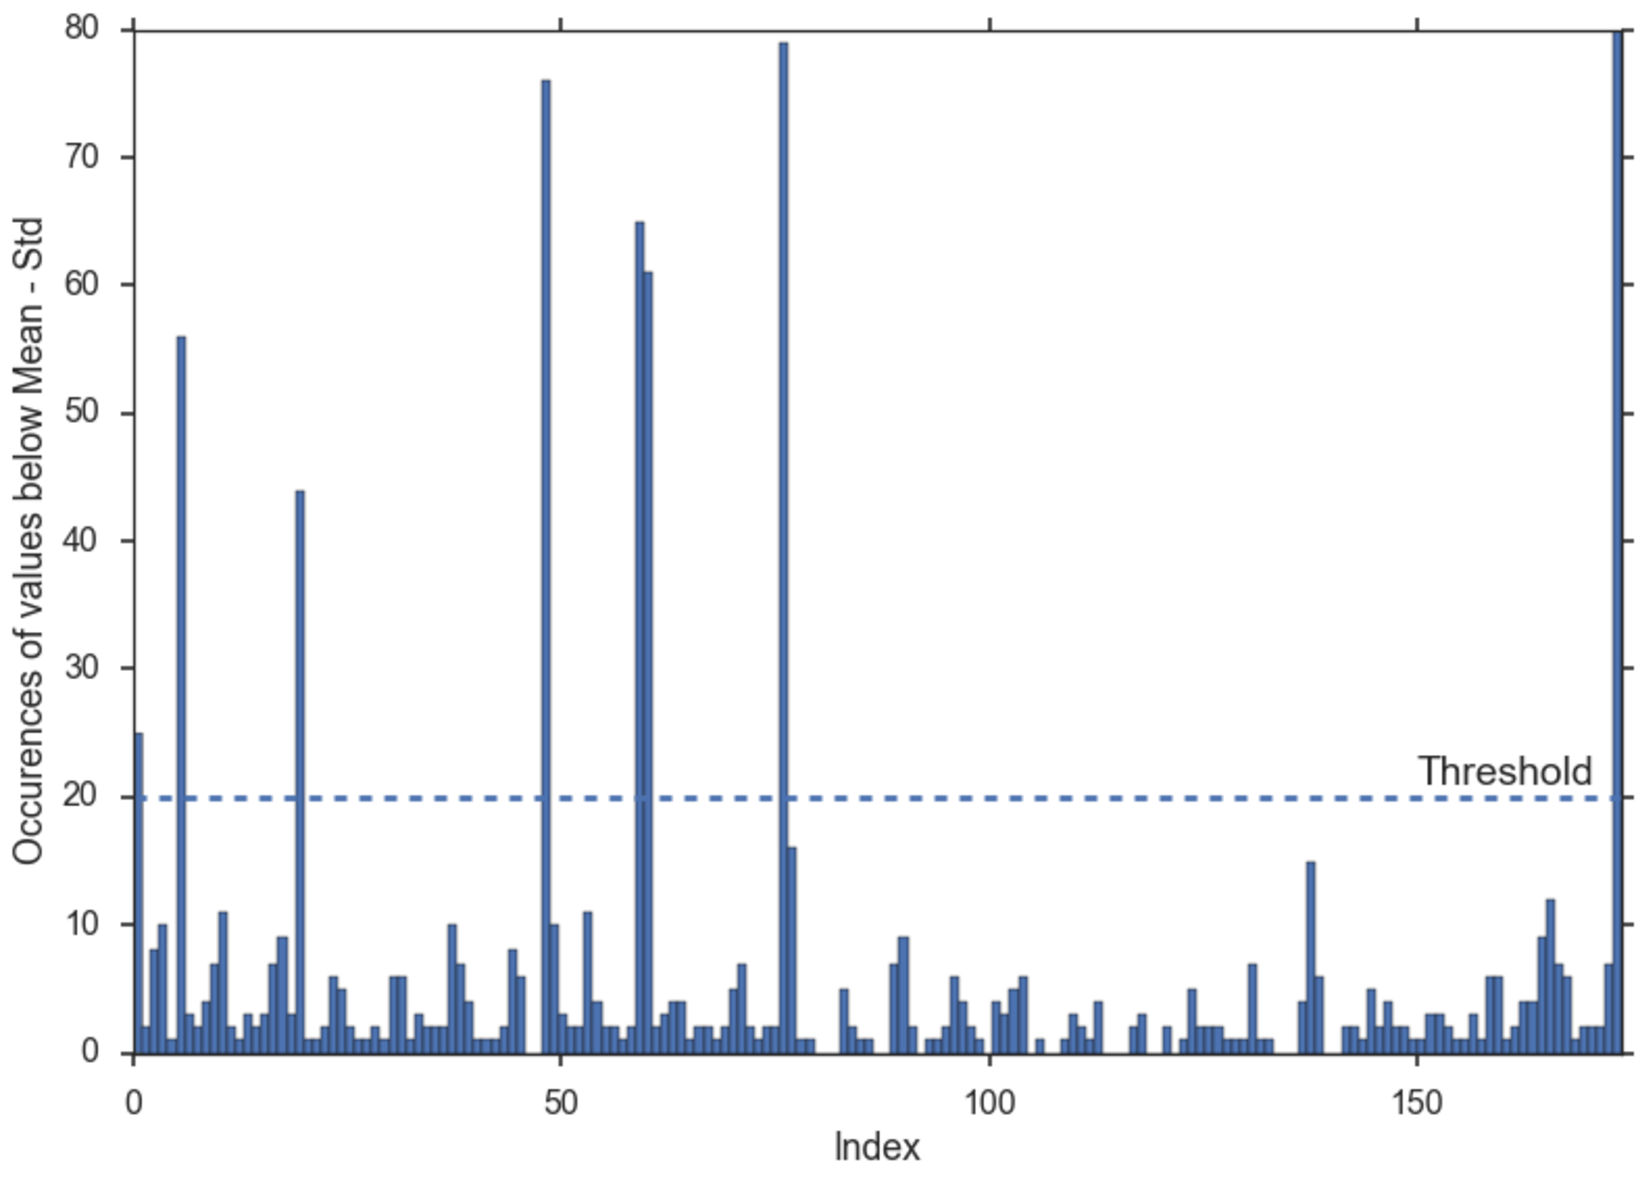
\includegraphics[width=\linewidth]{figs/incomplete_data.pdf}
\caption{Histogram of the occurences of specific indices, which correspond to individual days, for which the number of mentions of a keyword is below the average minus the standard deviation for this keyword. The threshold is set at 20.}
\label{fig:incomplete}
\end{figure}

The streaming of Twitter data was interrupted several times during the period the data were collected. Thus, minutes, hours, or even days are missing. While missing days are trivial to identify, doing so for partly incomplete daily data is more complicated. These days however would induce systematic biases to the analysis, as for all keywords the number of mentions decreases at the same time, thus inducing artificial strong positive correlations.

Without access to statistics on the streaming of the data, only an empirical correction on the reduced data set is possible. We proceed in the following way, we compute the mean and the standard deviation for the number of mentions over time for each keyword. We note the indices, which correspond to individual days, in these time series for which
\begin{equation}
\# \mathrm{Mentions} < \mathrm{Mean} - 1\cdot\mathrm{Std},
\end{equation}
and compare these indices among the keywords. We then set a threshold and consider the days incomplete, for which the number of occurences of the keyword is below the mean and standard deviation for at least 20 keywords. This process is illustrated in Figure~\ref{fig:incomplete}. 

In order not to bias our analysis by, we remove the occurences of the keywords for these days then from our analysis and treat them as days for which we do not have any tweets (see Section~\ref{sec:missingdata}).

All our analysis codes can be found on this public \textsc{GitHub} repository \cite{github}.

\section{Time series analysis}
The main results of the data reduction explained in the previous section, are time series of the occurrence of each of the 100 keywords in the queried twitter dataset. In order to identify relationships between different keywords, we compare their occurrence frequencies using two different methods based on the Pearson correlation coefficient. 

\subsection{Correlation between stationary time series}
We can determine the amount of linear dependence between two time series $X_{i}$ and $X_{j}$ using the correlation coefficient $\rho$. The correlation $\rho(\Delta t)$ between two time series is a function of the time lag $\Delta t$ between the two and is defined as \cite{dettling14}
\begin{equation}
\rho_{ij}(\Delta t) = \langle (X_{i, t}-\bar{X}_{i}) (X_{j, t+\Delta t}-\bar{X}_{j}) \rangle, \label{eq:corrcoef}
\end{equation} 
where $\langle ... \rangle$ denotes the ensemble average. For $\Delta t = 0$ we recover the usual correlation coefficient, whereas for $\Delta t \neq 0$, $\rho_{ij}(\Delta t)$ quantifies the amount of linear dependence between shifted time series. If the two time series are equal i.e. $i = j$, we recover the autocorrelation function of the time series, which quantifies the amount of linear dependence in the time series itself. In order to compare the correlation between different time series, it is customary to normalise Eq.~\ref{eq:corrcoef} by the variance of the two time series i.e. \cite{dettling14}
\begin{equation}
\rho_{ij}(\Delta t) = \frac{\langle (X_{i, t}-\bar{X}_{i}) (X_{j, t+\Delta t}-\bar{X}_{j}) \rangle}{\sqrt{\langle (X_{i, t}-\bar{X}_{i}) (X_{i, t}-\bar{X}_{i}) \rangle \langle (X_{j, t}-\bar{X}_{j}) (X_{j, t}-\bar{X}_{j}) \rangle}}. \label{eq:corrcoef1}
\end{equation} 

When performing time series analyses we generally do not have access to the ensemble averages of the series, but we need to estimate the auto and cross correlations from the samples we have at hand. In order to be able to estimate the auto- or cross correlation using Eq.~\ref{eq:corrcoef}, the ensemble average needs to equal the sample mean i.e. the values of both time series at all times $t$ need to identically distributed random variables. This is equivalent to requiring both time series $X_{i}$, $X_{j}$ to be stationary, which means that their mean $\mu$, variance $\sigma^{2}$ and autocorrelation function $\rho_{ii}(\Delta t)$ do not depend explicitly on time $t$
\begin{align}
\mu &= \langle X_{i, t} \rangle, \\
\sigma^{2} &=  \langle (X_{i, t}-\bar{X})^{2} \rangle \\
\rho_{ii}(\Delta t) &= \frac{\langle (X_{i, t}-\bar{X}_{i}) (X_{i, t+\Delta t}-\bar{X}_{i}) \rangle}{\sqrt{\langle (X_{i, t}-\bar{X}_{i}) (X_{i, t}-\bar{X}_{i}) \rangle \langle (X_{i, t+\Delta t}-\bar{X}_{i}) (X_{i, t+\Delta t}-\bar{X}_{i}) \rangle}}. 
\end{align} 
Only in this case, can we replace the ensemble averages in Equations \ref{eq:corrcoef} and \ref{eq:corrcoef1} with the sample means. This leads to the following estimators for the auto and cross correlation functions \cite{dettling14}:
\begin{align}
\rho_{ii}(\Delta t) &= \frac{\sum_{t=1}^{n-\Delta t} (X_{i, t}-\bar{X}_{i}) (X_{i, t+\Delta t}-\bar{X}_{i})}{\sum_{t=1}^{n} (X_{i, t}-\bar{X}_{i})^{2}} \\
\rho_{ij}(\Delta t) &= \frac{\sum_{t=1}^{n-\Delta t} (X_{i, t}-\bar{X}_{i}) (X_{j, t+\Delta t}-\bar{X}_{j})}{\sqrt{\sum_{t=1}^{n} (X_{i, t}-\bar{X}_{i})^{2}\sum_{t=1}^{n} (X_{j, t}-\bar{X}_{j})^{2}}}.
\end{align} 

\subsection{Differencing of non-stationary time series}
We do not expect the occurrences of keywords in twitter data to be stationary time series, since the mean occurrence of any keyword will for example depend on world events, its popularity and also on the number of people using twitter. We can roughly assess if any time series is stationary by visually inspecting the time series plot and also by computing its autocorrelation function $\rho(\Delta t)$. Non stationary time series are generally characterised by clear patterns in the autocorrelation functions because consecutive values are strongly correlated through the common trend.

In order to be able to quantify the correlation between non stationary time series we need to make the series stationary prior to evaluating Equations \ref{eq:corrcoef} and \ref{eq:corrcoef1}. The most basic form is called differencing, which allows us to transform time series with a slow trend to a stationary series. A time series with a trend can be written as \cite{dettling14}
\begin{equation}
X_{i, t} = T_{i, t} + R_{i, t},
\end{equation} 
where $T_{i, t}$ denotes the time series' trend and $R_{i, t}$ are random fluctuations around this trend. These fluctuations $R_{i, t}$ are generally correlated random variables with mean zero. If the time series varies slowly, we can remove the trend by considering the differenced time series instead of the initial one. The differenced time series is defined as \cite{dettling14}
\begin{equation}
D_{i, t} = X_{i, t+1}- X_{i, t}.
\label{eq:diff}
\end{equation} 
If $T_{i, t}$ is slowly varying, this transformed time series will only capture the random variations around the global trend and will thus approximately be stationary.

For non stationary time series, we can thus first perform differencing and then compute the auto and cross correlations between the differenced time series. This will encode the amount of linear dependence between changes in one time series from its global trend and changes in the second. 

In order to quantify the significance of both the auto- and cross correlations, we need to compare the measured values to the expected values for uncorrelated time series. For uncorrelated time series, which are a sequence of IID variables we expect both for the auto and cross correlations $\rho(\Delta t) = 0$ with a variance of $\sigma^{2}(\rho(\Delta t)) = \frac{1}{n}$, where $n$ denotes the number of samples used to estimate the correlation \cite{dettling14}. For simplicity, we will call a cross-correlation between two time series significant if its value exceeds $1.96 \sigma(\rho(\Delta t))$ (i.e. the $95 \%$ confidence limits), even though we do not expect the differenced time series to be perfect IID processes. 

\subsection{Missing data}\label{sec:missingdata}
The above considerations assume that there is no missing time series data, which is rarely the case in reality. Several pieces of data are missing in the twitter dataset. First of all we do not have access to data for most of August 2014 and furthermore there are several days missing throughout. In order to be able to analyse the data, we therefore fill the missing values using random samples drawn from a normal distribution with the mean and variance of the respective time series. This procedure will keep mean and standard deviation constant and will not introduce any correlations between different time series.

In order to find relations between keywords, we will proceed in two steps: for illustration purposes we will compute the cross correlation between all the time series (filled as explained above) regardless of stationarity for timelags $-10 \leq \Delta t \leq 10$. We will then compute the autocorrelation function of all the series and recompute the correlation coefficients using the differenced time series for non stationary processes. For both methods, we assign the highest correlation coefficient (regardless of timelag $\Delta t$) to each pair and compare the results obtained with these two measures. 

\section{Results}
The occurrence of different keywords over time displays different behaviour depending on the keyword. Keywords from the everyday life and family sections for example feature stationary time series with little to no variation. On the other hand, keywords associated to major events show significant trends and structure. Examples for both these cases are shown in Figures \ref{fig:timeseries_abs} and \ref{fig:timeseries_rel}. Please see Figure 5 in the results section on http://spuriousrelationships.eu.pn/ for the time series of all our keywords. Figures \ref{fig:timeseries_abs} and \ref{fig:timeseries_rel} show the absolute and relative time series for the words \textit{banana} and \textit{MH17} respectively. \textit{MH17} is the abbreviation for the Malaysian airlines flight 17, which was shot down over the Ukraine on July, 17th 2014. We see that the mentions of \textit{MH17} are concentrated in this period while the word banana appears with a constant frequency over the 6 months we have analysed. The time series for the word \textit{apple} is an example for the occurrence frequency of words with different meanings as detailed in Section \ref{sec:data}. The word \textit{apple} refers to both the fruit as well as the company. We would expect the frequency of the fruit to be fairly time-independent, but from Figures \ref{fig:timeseries_abs} and \ref{fig:timeseries_rel}, we see that the number of mentions features a strong peak in September, 2014. This is probably caused by apple holding its keynote speech on September 9th, 2014, showing that different word usages can dominate the occurrence frequency at different times.

\begin{figure}
\centering
\begin{subfigure}{.5\textwidth}
  \centering
  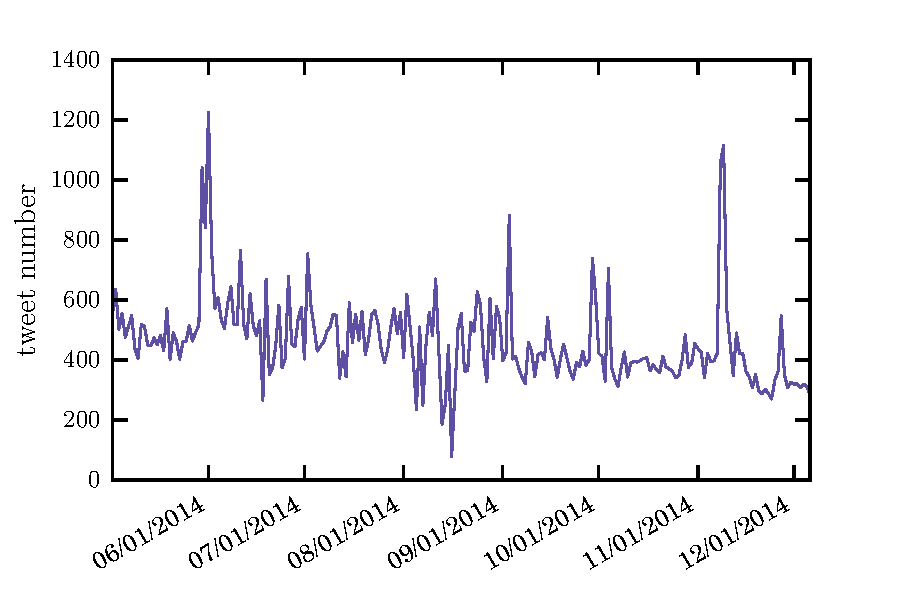
\includegraphics[width=.9\linewidth]{figs/banana_absolute.pdf}
  \caption{Occurrence frequency for \textit{banana}.}
  \label{fig:sub11}
\end{subfigure}%
\begin{subfigure}{.5\textwidth}
  \centering
  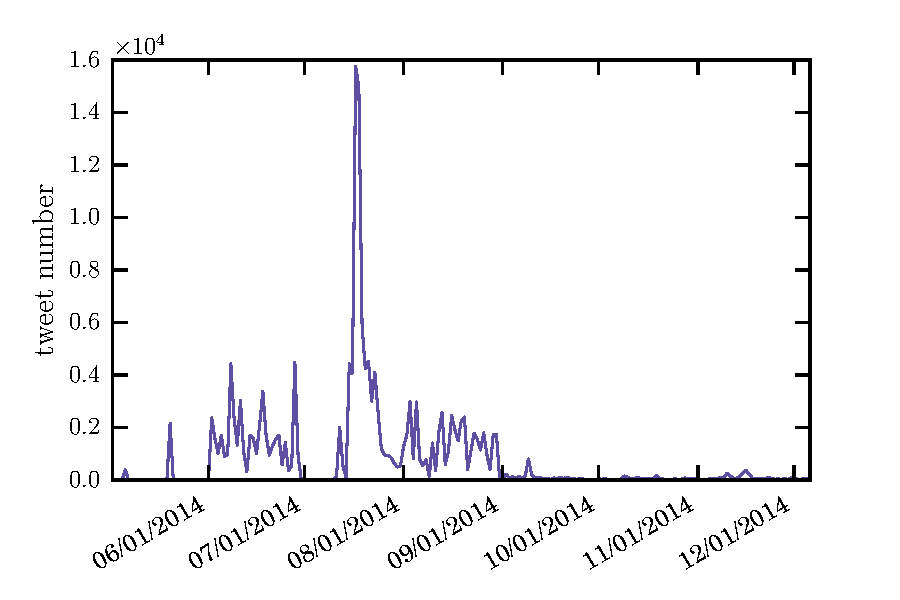
\includegraphics[width=.9\linewidth]{figs/mh17_absolute.pdf}
  \caption{Occurrence frequency for \textit{MH17}.}
  \label{fig:sub12}
\end{subfigure}
\begin{subfigure}{.5\textwidth}
  \centering
  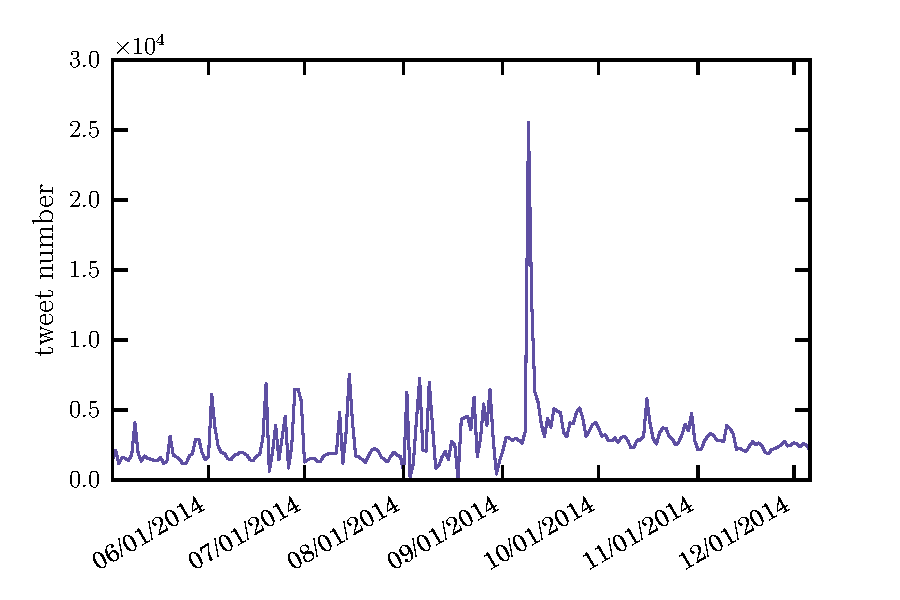
\includegraphics[width=.9\linewidth]{figs/apple_absolute.pdf}
  \caption{Occurrence frequency for \textit{apple}.}
  \label{fig:sub13}
\end{subfigure}
\caption{Absolute number of keyword occurrences as a function of time.}
\label{fig:timeseries_abs}
\end{figure}

\begin{figure}
\centering
\begin{subfigure}{.5\textwidth}
  \centering
  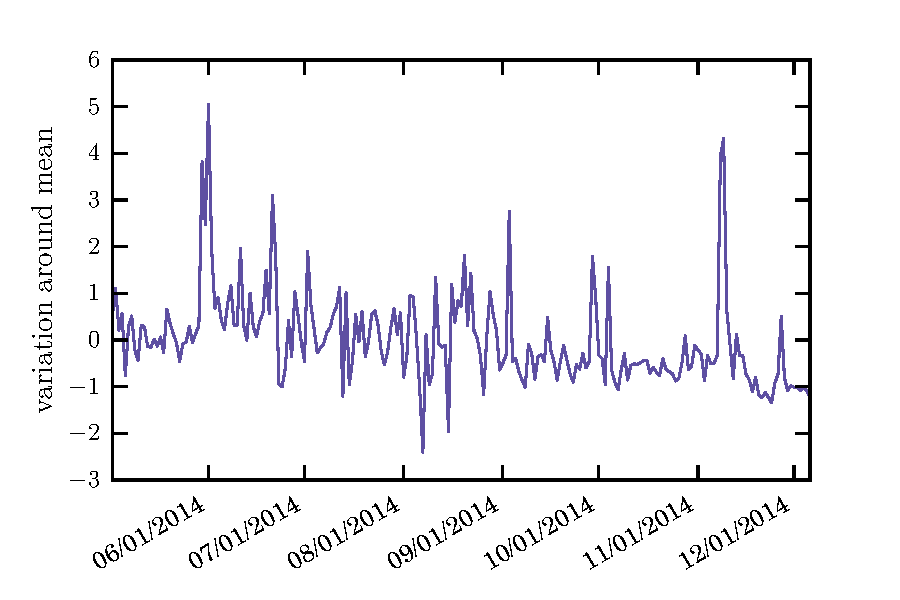
\includegraphics[width=.9\linewidth]{figs/banana.pdf}
  \caption{Occurrence frequency for \textit{banana}.}
  \label{fig:sub21}
\end{subfigure}%
\begin{subfigure}{.5\textwidth}
  \centering
  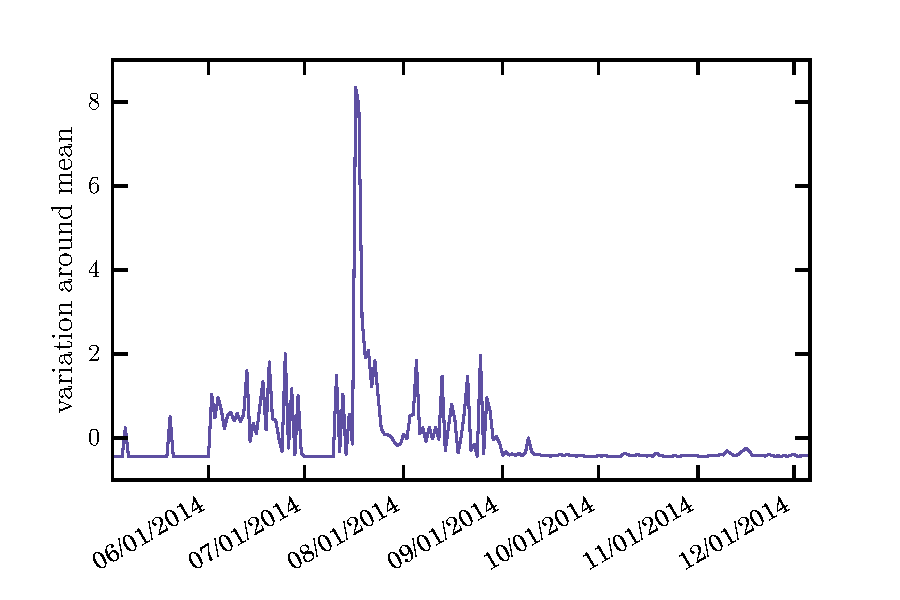
\includegraphics[width=.9\linewidth]{figs/mh17.pdf}
  \caption{Occurrence frequency for \textit{MH17}.}
  \label{fig:sub22}
\end{subfigure}
\begin{subfigure}{.5\textwidth}
  \centering
  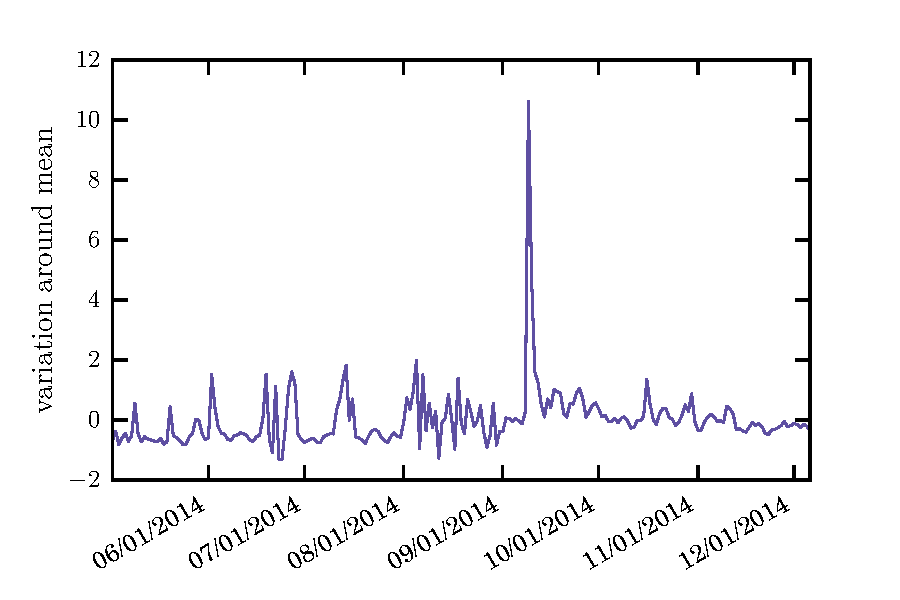
\includegraphics[width=.9\linewidth]{figs/apple.pdf}
  \caption{Occurrence frequency for \textit{apple}.}
  \label{fig:sub23}
\end{subfigure}
\caption{Mean subtracted number of keyword occurrences as a function of time normalised by the standard deviation of the time series.}
\label{fig:timeseries_rel}
\end{figure}

From Figures \ref{fig:timeseries_abs} and \ref{fig:timeseries_rel}, we see that in general, the time series are not stationary. We therefore transform all the time series by differencing, as outlined in Eq.~\ref{eq:diff}. The differenced time series for the keyword \textit{MH17} are shown in Fig.~\ref{fig:diff_acf} along with its autocorrelation function. We see that the differenced time series is significantly more stationary, even though \textit{MH17} is one of the most strongly varying keywords in our sample. This is confirmed by the autocorrelation function.

The cross correlation coefficients between keyword pairs for both methods are shown in Figures 6 and 7 on http://spuriousrelationships.eu.pn/. As expected, we see a correlation of 1 on the diagonal, corresponding to the normalised auto correlations. The correlation matrix has a block-diagonal form corresponding to the correlations within keyword groups, e.g. keywords within the refugees and terrorism categories. Comparing the two correlation measures, we find that the correlations computed from the differenced time series are less pronounced than the ones computed using the raw data. This is expected, since the latter method generally overestimates correlations. 

\begin{figure}
\centering
\begin{subfigure}{.5\textwidth}
  \centering
  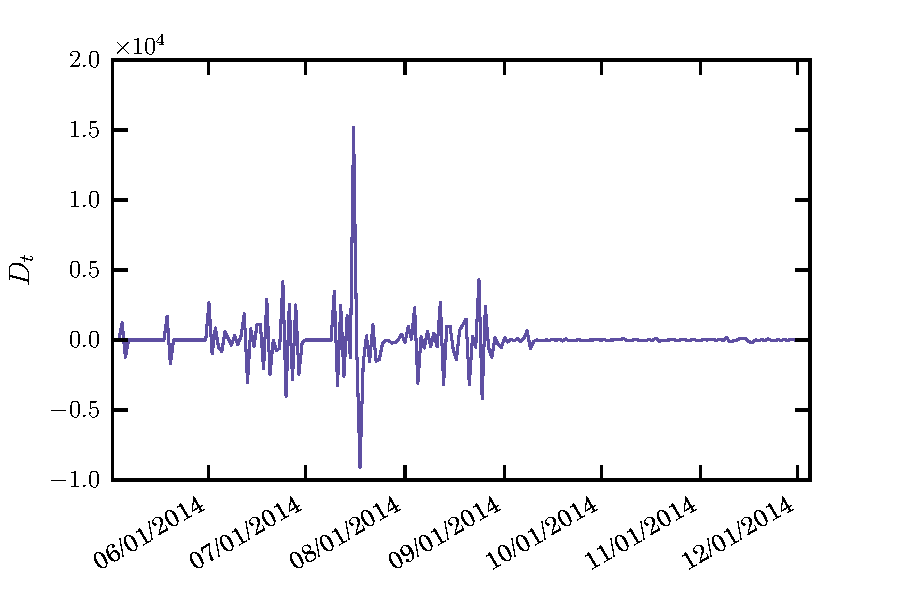
\includegraphics[width=.9\linewidth]{figs/mh17_diff.pdf}
  \caption{Differenced time series for \textit{MH17}.}
\end{subfigure}%
\begin{subfigure}{.5\textwidth}
  \centering
  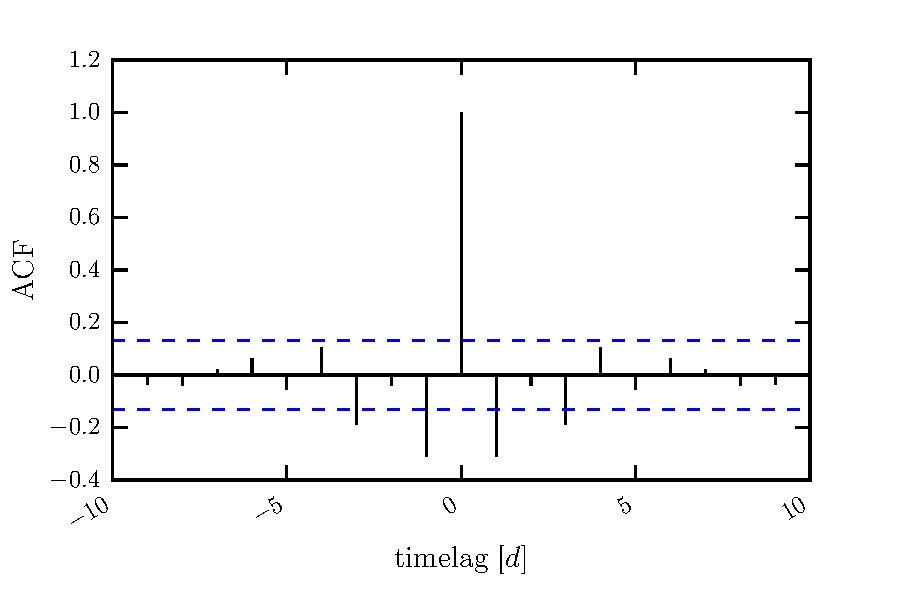
\includegraphics[width=.9\linewidth]{figs/mh17_acf.pdf}
  \caption{Autocorrelation function for \textit{MH17}.}
\end{subfigure}
\caption{Differenced time series and autocorrelation function for \textit{MH17}. The dashed lines indicate $95 \%$ confidence intervals for IID data.}
\label{fig:diff_acf}
\end{figure}

As can be seen from these figures, we are able to retrieve expected correlations, such as correlation between \textit{nelson} and \textit{mandela} or \textit{refugees} and \textit{syria}. However, we also find several unexpected and probably spurious correlations between keywords such as \textit{maya} and \textit{television} or \textit{mandela} and \textit{ukraine}. 
This is probably both due to the simple methods employed to compute correlations as well as that computing correlations between noisy datasets without clear features is generally a difficult problem. Table \ref{tab:example_corr} shows further examples of expected and unexpected correlations and non-correlations.

\begin{minipage}{\linewidth}
	\centering
	\captionof{table}{Examples of expected and unexpected correlations and non-correlations}\label{tab:example_corr} 
	\begin{tabular}{ | l | l || l | l |}
		\hline
		Expected Correlation &  & Expected Non-correlation & \\ \hline
		Keywords & Value & Keywords & Value \\ \hline
		$nelson$ \& $mandela$ & 0.793 & $climate$ \& $banana$ & 0.193\\
		$MH17$ \& $ukraine$ & 0.713 & $whatsApp$ \& $jogging$ & -0.175\\
		$refugees$ \& $syria$ & -0.218 & $wedding$ \& $ukraine$ & 0.685\\ \hline \hline
		
		Unexpected Correlation &  & Unexpected Non-correlation & \\ \hline
		Keywords & Value & Keywords & Value \\ \hline
		$nelson$ \& $pig$ & 0.719 & $attack$ \& $terrorism$ & -0.186\\
		$maya$ \& $flu$ & 0.802 & $snowden$ \& $russia$ &  0.146\\
		$isis$ \& $rosetta$ & -0.562 & $refugees$ \& $asylum$ & 0.685\\ \hline
	\end{tabular}
	% \par
\end{minipage}


\section{Conclusion}
In this project we analysed roughly six months of unfiltered twitter data by querying the tweets for a set of 100 predefined keywords. We aimed at recovering correlations between the occurrence frequencies of related keywords and showing that spurious relationships can be detected in large datasets. We used both the time series of the number of tweets per day containing a particular keyword and its differenced counterpart to compute correlation coefficients for pairs of keywords. 

While we found large correlation coefficients for \textit{a priori} expected keyword pairs, we also measured a significant number of unexpected and probably spurious correlations. This shows that large data sets need to be carefully analysed and that the increasing volume of data sets asks for exploration of novel analysis methods.


\section{Acknowledgements}
This project was part of the lecture \textit{Data Science in Techno-Socio-Economic Systems} given by Dr. Evangelos Pournaras, Prof. Dr. Dirk Helbing and Dr. Izabela Moise at ETH Zurich during the spring semester 2016. We would like to thank Dr. Izabela Moise and Dr. Rok Roskar for the valuable guidance and helpful discussions. We used \textsc{Apache Spark} \cite{spark}  to query the Twitter data, and \textsc{Python} \cite{python} and \textsc{bokeh} \cite{bokeh} for the data analysis and visualization. The website was built on a \textsc{html5up} \cite{html5up} template.

\begin{thebibliography}{9}

\bibitem{tyler_vigen}
\url{http://tylervigen.com/spurious-correlations}
\bibitem{webpage}\url{http://spuriousrelationships.eu.pn/}
\bibitem{twitter}\url{https://twitter.com/}
\bibitem{facebook}\url{https://www.facebook.com/}
\bibitem{reddit}\url{https://www.reddit.com/}
\bibitem{twitterstream}\url{https://dev.twitter.com/streaming/public}
\bibitem{rosetta}\url{http://www.esa.int/Our_Activities/Space_Science/Rosetta}
\bibitem{who}\url{http://www.who.int/en/}
\bibitem{pyspark}\url{https://spark.apache.org/}
\bibitem{github}\url{https://github.com/cbruderer/spuriousrelations}
\bibitem{dettling14} Marcel Dettling, Applied Time Series Analysis, SS 2014, Zurich University of Applied Sciences, \url{https://stat.ethz.ch/education/semesters/ss2014/atsa/Scriptum_v140523.pdf}
\bibitem{spark}\url{http://spark.apache.org}
\bibitem{python}\url{https://www.python.org}
\bibitem{bokeh}\url{http://bokeh.pydata.org/en/latest/}
\bibitem{html5up}\url{http://html5up.net}

\end{thebibliography}

\end{document}
